\documentclass[journal]{IEEEtran}

\usepackage{biblatex}

\usepackage[fleqn]{amsmath}
\usepackage{amssymb}
\usepackage{graphicx}
\usepackage{cancel}
\addbibresource{./citations.bib}

% \graphicspath{ {C:/Users/jonat/Documents/ECH-267-Adv.-Proc.-Control/Project/1_Report/images/}}
\graphicspath{ {C:/Users/Indy-Windows/Documents/ECH-267-Adv.-Proc.-Control/Project/1_Report/images/}}

\usepackage{hyperref}
\hypersetup{
colorlinks=false,
linkcolor=blue,
filecolor=magenta,
    urlcolor=blue,
}
\urlstyle{same}

% \hyphenation{op-tical net-works semi-conduc-tor}


\begin{document}

\title{MPC for Robotic Arm Path Planning and Control \\ ECH-267 Final Project Report}


\author{Jonathan~Dorsey \IEEEmembership{Member: No Sleep Club: est. 2017} \\  \url{https://github.com/JonnyD1117/ECH-267-Adv.-Proc.-Control/tree/main/Project}}


% The paper headers
\markboth{Journal of Graduate School Assignments, March~2021}%
{Dorsey \MakeLowercase{\textit{et al.}}: MPC for Robotic Arm Path Planning and Control ECH-267 Final Project Report}

% make the title area
\maketitle

% As a general rule, do not put math, special symbols or citations
% in the abstract or keywords.
\begin{abstract}
  The objective of this project is to implement a simulated optimal \underline{Path Planner} using Model Predictive Control (MPC) to plan and control the behavior of a 2 degree of freedom (2DOF) robotic arm. The responsibility of the MPC planner will be to generate the `optimal' path and to drive the arm from its current position to the next. The main challenges faced in completing this project consist of solving for the \textbf{nonlinear equations of motion} (as well as any required forward/inverse kinematics) of the robotic arm as well as formulating and solving the \textbf{MPC controller}, at each timestep, both control and planning using the CasADi optimization framework, to test the scenario of simulated real-time performance.
\end{abstract}

% Note that keywords are not normally used for peerreview papers.
\begin{IEEEkeywords}
Model Predictive Control, Robot Arm, Lagrange Equations, Path Planning, Obsticle Avoidance, DH Parameters, Trajectory Generation.
\end{IEEEkeywords}


\IEEEpeerreviewmaketitle

\section{Introduction}

\IEEEPARstart{T}{he} world of robotics is full of constraints, demands, and performance trade-offs that humans handle naturally on a daily basis. Unlike humans, robots require control and planning strategies which are flexibility enough to work around constraints and limitations, while accurately meeting control and performance objectives in uncertain environments. While the emergence of machine learning techniques and methods offers promise of stateoftheart improvements and performance, most robotic systems still demand a more practical and robust planning and control algorithms, capable of offering a compromise between the performance criteria, flexibility to navigate constraints, and amount of computational power required to compute valid control commands in real-time. \\

In the world of robot manipulators, tasks can range from relatively simple and coarse motions to extremely complex and detailed actions. One common control strategy which has seen great success, in robotics, in recent years is Model Predictive Control (MPC). MPC is an optimal control methodology which solves the a given optimal control problem (OCP) in a receding fashion, over a finite horizon. While these controllers are far more sophisticated than standard classical or modern control strategies, the increased complexity and computation can be applied to a wider class of control problems. This flexibility in natively handling constraints as well as naturally extending to nonlinear and multiple-input-multiple-output-systems makes MPC an attractive candidate control methodology for the vast world of robotics where tasks can range from autonomous mobile vehicles to robotic manipulators. While MPC has the obvious conns of requiring an approximate solution to an optimization problem, at each time step, the benefits which this methodology offers often make it a viable solution even with the added computationally expense. \\

While control is an important aspect of modern robotics, it is often more valuable to have an understanding of the intent or future actions which an autonomous system believes it should take, to accomplish a goal. In general, this problem is known as \textbf{path planning}, and is an important part of modern robotics research. Many modern path planning approaches use a vast array of different planning paradigms, such as discretization, graph, probablistic, and heuristic methods which have all shown great promise, and present there own unique benefits and limitations. Often in the more general case of motion planning, it is desirable to not only control the position, but also the velocity and acceleration of a system, in both space and time. However, for the purpose of this paper, only the more restricted case of path planning (e.g. position planning) will be considered.  \\

To this point, another possible method for path planning is the use of MPC, as a optimal path planner. MPC has the potential to provide much of the same functionality as other planning strategies by implementing desireable behavior into a cost function or functional constraints. The ability to leverage and model predictive controller as a path planning with practically no changes to its implementation as a controller also offers an opportunity for systems using MPC to obtain some path planning capabilities for free.   \\

While MPC has been received enormous amounts of research across many fields, including  robotics, many of the applications in robotics focus MPC on mobile robotics such as drones and autonomous vehicles, with significantly less attention focused on the application of MPC as a controller or a planner for robotic manipulators.

This paper will investigate the use of MPC as a general control methodology and its viability as a path planner for a simple two link planar robotic manipulator. By running simulate tests, this paper plans to develop an understanding about the general benefits and limitations of MPC in the context of articulated robotics.   


\section{Problem Statement}

1 investigate the benefits and drawbacks of control using MPC on robot

    USECASE: Full MPC control over robot arm

2 Investigate the benefits and drawbacks of path planning using MPC on robot

    USECASE: MPC as optimal path planner for external control of robot arm


\section{Background}

\subsection{Robotics}

\subsubsection{}

\subsubsection{}

\subsubsection{}


\subsection{}


\section{Methodology}

\subsection{Formulation of Robot Dynamics}
1 Formulate Dynamics Model

\subsection{MPC Formulation}
2 Define appropriate MPC problem

\subsubsection{Cost Function Design}

2.1 Cost Function Definition
  2.1.1 Pose to Pose
  2.1.2 Obstacle Avoidance


\subsection{Develop Symbolic Model in CasADi}
3 Define CasADi Model



\subsection{Controller \& Planner Simulation}
4 Simulate Model \& Model Predictive Controller in Matlab



\subsection{Controller Testing}

5 Test MPC as Controller
    5.1 MIMO pose to pose Controller
    5.2 Controller with Model/Parameter Mismatch
    5.3 Limited Position Constraints
    5.4 Obstacle avoding controller


\subsection{Planner Testing }

6 Test MPC as Path Planner
    6.1 Generate Optimal State Prediction over horizon
    6.2 Use Cubic Splines to define a continuous path from end effector ``start'' position to end effector ``end'' position.
    6.3 Use a faster controller to follow path that MPC generated Path predicts

6.1 Test MPC generated Path with Fullstate Feedback Controller


\section{Results}

\subsection{Controller Results}




\subsection{Planner Results}


\section{Discussion}

\subsection{Control}

0 Fully controllable environment \\
1 MIMO formulation is intuitive \& easily extended to nonlinear systems (2D-3D)\\
2 Relatively responsive control authority\\
3 Respects system constraints (Actuator limits, range of motions)\\
4 Relatively simple to implement a crude form of obstacle avoidance (cost penalty or extra constriants.)\\
    4.1 Unreliable time till solution\\
    4.2 Highly sensitive to obstacle placement\\
    4.3 Poor tuning can lead to oscilatory behavior\\
    4.4 Can struggle to converge to final solution even if clear of obstacle (tuning?)\\
5

\subsection{Planning}

Possible To use MPC as a supervisory controller/planner for other\\

MPC planner is able to update the best path (given the current state) and can account for model uncertainties or object/obstacles in the direct path.\\

Planning with MPC allows the planner to track smoothly though the optimal state horizon which can then be leveraged by other controllers ...etc. which function at faster speeds than the base MPC controller could.\\

Unlike the most commonly used path planning algorithms (A*, Djikstra, RRT, RRT*, PRM, D*, and other discretized, graph, or heuristic search algorithms, such as Artifial potential fields) Path planning with MPC is a very control theoretic approach.\\

While the use case seen in this paper is not very impressive, predicting and controlling the path which the end effector of a robot takes from one position to another can quicker be seen in the three dimensional case where discretizing the entire feasible can be computationally intensive.\\





\section{Conclusion}
The conclusion goes here.


\section*{Acknowledgment}


The authors would like to thank Mountain Dew and his matress for constant support and comfort.



\ifCLASSOPTIONcaptionsoff
  \newpage
\fi

\cite{craig_introduction_2005}
\cite{khalil_nonlinear_2002}
\cite{rawlings_model_2017}
\cite{armstrong_explicit_1986}
\cite{ogata_modern_2010}
\cite{meriam_engineering_1993}
\cite{greenwood_advanced_2006}
\cite{borrelli_predictive_2017}
\cite{boyd_convex_2004}
\cite{slotine_applied_1991}
\cite{soft_constraints}

% \printbibliography

\begin{IEEEbiography}[{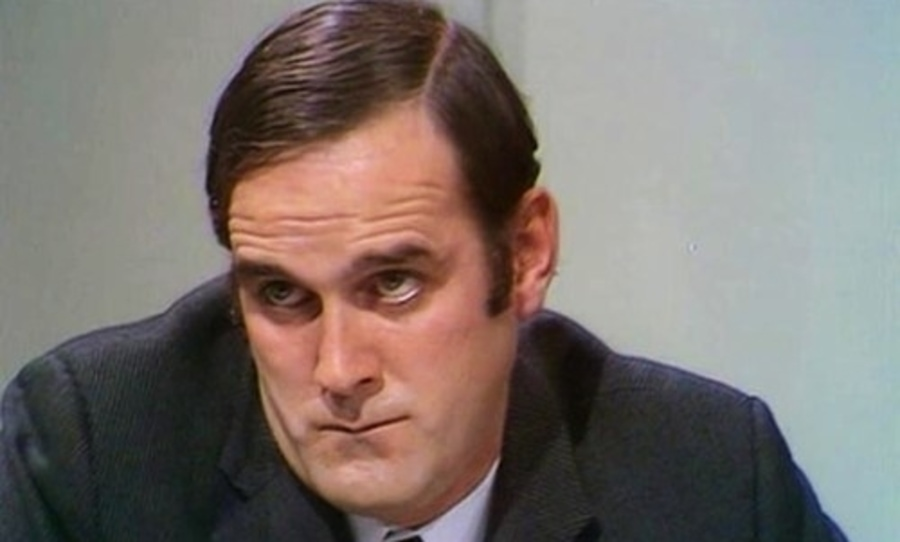
\includegraphics[width=1in,height=1.25in,clip,keepaspectratio]{monty1}}]{Jonathan Dorsey}
  I've already told you once. It is an ex parrot. Its has ceased to be. Recieved his Bachelors Degree in Mechanical Engineering from the San Jose State University. With a focus on mechatronics and control systems, he has developed an interest in reinforcement learning, computer vision, and control and design of autonomous systems.
\end{IEEEbiography}



\end{document}
